%%%%%%%%%%%%%%%%%%%%%%%%%%%%%%%%%%%%%%%%%%%%%%%%%%%%%%%%%%%%%%%%%%%%%%%%
% Escuela Politécnica Superior de la Universidad de Alicante
% Realizado por: Jose Manuel Requena Plens
% Contacto: info@jmrplens.com / Telegram:@jmrplens
%%%%%%%%%%%%%%%%%%%%%%%%%%%%%%%%%%%%%%%%%%%%%%%%%%%%%%%%%%%%%%%%%%%%%%%%

\definecolor{mycolor1}{rgb}{1.00000,0.00000,1.00000}%
%
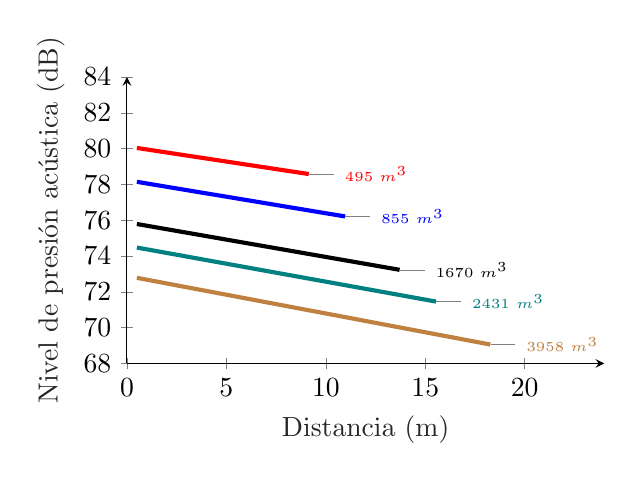
\begin{tikzpicture}

\begin{axis}[%
width=0.5\textwidth,
height=0.3\textwidth,
at={(0\textwidth,0\textwidth)},
scale only axis,
xmin=0,
xmax=24,
xlabel style={font=\color{white!15!black}},
xlabel={Distancia (m)},
ymin=68,
ymax=84,
ytick distance=2,
axis y line=left,
axis x line=bottom,
cycle list name=color list,
ylabel style={font=\color{white!15!black}},
ylabel={Nivel de presión acústica (dB)},
axis background/.style={fill=white},
legend style={legend cell align=left, align=left, draw=white!15!black}
]

% Campos utiles

% 1
\addplot+[ line width=1.5,domain=0.5:9.14, samples=10,every node/.style={xshift=-4pt}]
{10*log10(1.0337e+12 * ( (4*0.0026389378)/(512*(-ln(1-0.1176))) * e^(-(13.82*((x/343)+0.05)*1.195 / 1.24))*1.175))} node [pos=1,pin=0:{\tiny{495 $m^3$}}] {};

% 1.2
\addplot+[ line width=1.5,domain=0.5:10.97, samples=10,every node/.style={xshift=-4pt}]
{10*log10(1.0337e+12 * ( (4*0.0026389378)/(737*(-ln(1-0.1176))) * e^(-(13.82*((x/343)+0.05)*1.309 / 1.24))*1.168))} node [pos=1,pin=0:{\tiny{855 $m^3$}}] {};

% 1.5
\addplot+[ line width=1.5,domain=0.5:13.71, samples=10,every node/.style={xshift=-4pt}]
{10*log10(1.0337e+12 * ( (4*0.0026389378)/(1152*(-ln(1-0.1176))) * e^(-(13.82*((x/343)+0.05)*1.373 / 1.24))*1.101))} node [pos=1,pin=0:{\tiny{1670 $m^3$}}] {};

%% 1.7
\addplot[line width=1.5,color=teal, domain=0.5:15.54, samples=10,every node/.style={xshift=-4pt}]
{10*log10(1.0337e+12 * ( (4*0.0026389378)/(1479*(-ln(1-0.1176))) * e^(-(13.82*((x/343)+0.05)*1.422 / 1.24))*1.074))} node [pos=1,pin=0:{\tiny{2431 $m^3$}}] {};

% 20
\addplot+[ line width=1.5,domain=0.5:18.27, samples=10,every node/.style={xshift=-4pt}]
{10*log10(1.0337e+12 * ( (4*0.0026389378)/(2048*(-ln(1-0.1176))) * e^(-(13.82*((x/343)+0.05)*1.486 / 1.24))*1.045))} node [pos=1,pin=0:{\tiny{3958 $m^3$}}] {};


\end{axis}
\end{tikzpicture}%



